\chapter{क्रियात्मक समूह और परिवार}\label{ch:g11:functional-groups}

सिरके की एक बोतल, नेल पॉलिश रिमूवर की एक बोतल, नाशपाती वाली टॉफ़ियों का एक थैला
खोलिए, और मछली वाले की दुकान के पास से गुज़रिए: चार गंधें, तीखी, मीठी-विलायक
जैसी, फलों जैसी और मछली जैसी, और चार अलग-अलग प्रकार के \omterm{def:g7:atoms-and-molecules:molecule}{अणु}। हर एक की गंध, और
उसका ज़्यादातर रसायन, उसके कार्बन कंकाल के कारण नहीं, बल्कि उससे जुड़े \omterm{def:g7:atoms-and-molecules:atom}{परमाणुओं}
के एक छोटे समूह के कारण है: एक जगह ऑक्सीजन और हाइड्रोजन, दूसरी जगह एक नाइट्रोजन
\omterm{def:g7:atoms-and-molecules:atom}{परमाणु}। रसायनज्ञ \omterm{def:g11:organic-skeletons:organic}{कार्बनिक यौगिकों} को इन्हीं समूहों के अनुसार
छाँटते हैं।

\begin{recall}
\omterm{def:g11:organic-skeletons:formulas}{कंकाल सूत्र}, \omterm{def:g11:organic-skeletons:alkane}{ऐल्केनों} और \omterm{def:g11:organic-skeletons:alkane}{ऐल्किल समूहों} के नाम, \omterm{def:g11:organic-skeletons:isomer}{समावयवी}
(\cref{ch:g11:organic-skeletons})। \omterm{def:g11:polarity-and-cohesion:polar-bond}{ध्रुवीय आबंध} और \omterm{def:g11:polarity-and-cohesion:hydrogen-bond}{हाइड्रोजन आबंध}
(\cref{ch:g11:polarity-and-cohesion})।
\end{recall}

\begin{omfigure}
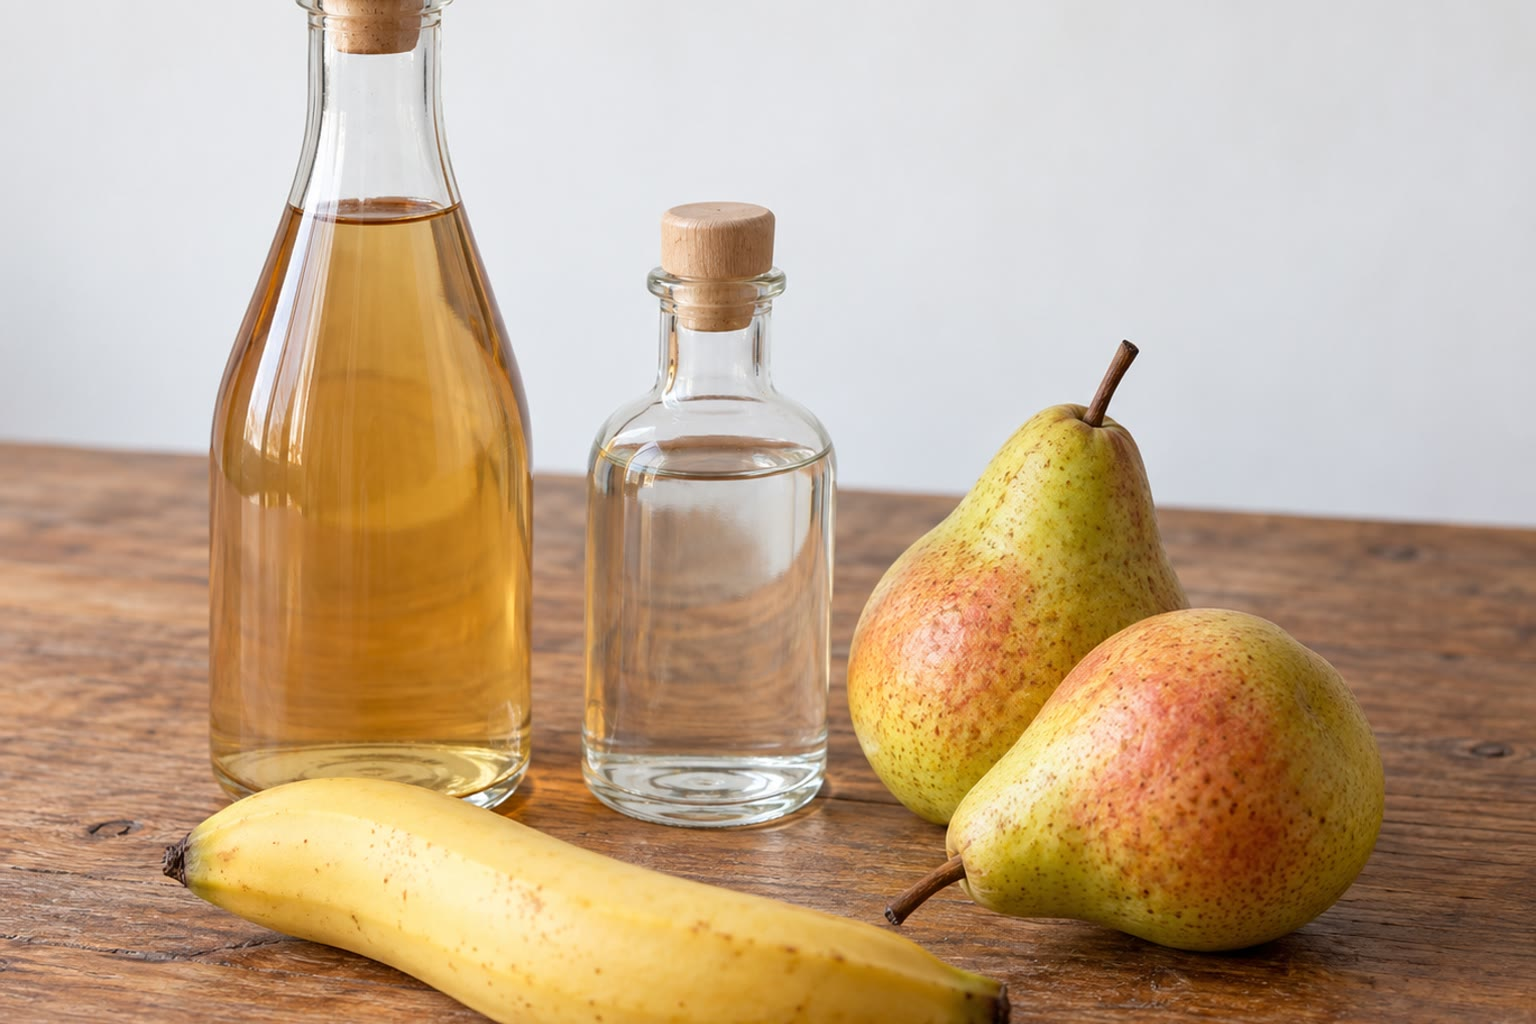
\includegraphics[width=0.5\linewidth]{images/book1/ai/g11-still-life-esters.jpg}

{\small सिरका, एक \omterm{def:g6:solutions-and-solubility:solute}{विलायक}, फल: हर गंध कार्बन कंकाल पर लगे \omterm{def:g7:atoms-and-molecules:atom}{परमाणुओं} के एक अलग
समूह से आती है।}
\end{omfigure}

\section{क्रियात्मक समूह}

\begin{definition}[क्रियात्मक समूह]\label{def:g11:functional-groups:functional-group}
\emph{क्रियात्मक समूह}\index{क्रियात्मक समूह} \omterm{def:g7:atoms-and-molecules:atom}{परमाणुओं} का ऐसा समूह है, जो
केवल एकल आबंधों से जुड़े कंकाल के कार्बन और हाइड्रोजन \omterm{def:g7:atoms-and-molecules:atom}{परमाणुओं} से अलग हो,
और \omterm{def:g7:atoms-and-molecules:molecule}{अणु} को उसकी अभिलाक्षणिक अभिक्रियाएँ दे। एक ही क्रियात्मक समूह वाले
यौगिक एक परिवार बनाते हैं।
\end{definition}

\begin{omfigure}
\renewcommand{\arraystretch}{1.35}
\footnotesize
\begin{tabular}{@{}l@{\enspace}l@{\enspace}l@{\enspace}l@{\enspace}l@{}}
\hline
समूह & सूत्र & परिवार & नाम का अंत & उदाहरण \\
\hline
हाइड्रॉक्सिल & \ce{-OH} & \omterm{def:g11:functional-groups:alcohol}{ऐल्कोहॉल} & \emph{-ऑल} & एथेनॉल, \ce{CH3-CH2-OH} \\
कार्बोनिल (सिरे पर) & \ce{-CHO} & \omterm{def:g11:functional-groups:carbonyl}{ऐल्डिहाइड} & \emph{-ऐल} & एथेनैल, \ce{CH3-CHO} \\
कार्बोनिल (भीतर) & \ce{C-CO-C} & \omterm{def:g11:functional-groups:carbonyl}{कीटोन} & \emph{-ओन} & प्रोपेनोन, \ce{CH3-CO-CH3} \\
कार्बोक्सिल & \ce{-COOH} & \omterm{def:g11:functional-groups:carboxylic-acid}{कार्बोक्सिलिक अम्ल} & \emph{-ओइक अम्ल} & एथेनोइक अम्ल, \ce{CH3-COOH} \\
\omterm{def:g11:functional-groups:carboxylic-acid}{एस्टर} & \ce{C-COO-C} & \omterm{def:g11:functional-groups:carboxylic-acid}{एस्टर} & \emph{-इल \ldots-ओएट} & एथिल एथेनोएट, \ce{CH3-COO-CH2-CH3} \\
\omterm{def:g11:functional-groups:amine}{ऐमीन} & \ce{-NH2} & \omterm{def:g11:functional-groups:amine}{ऐमीन} & \emph{-ऐमीन} & एथेनेमीन, \ce{CH3-CH2-NH2} \\
\omterm{def:g11:functional-groups:amine}{ऐमाइड} & \ce{-CONH2} & \omterm{def:g11:functional-groups:amine}{ऐमाइड} & \emph{-ऐमाइड} & एथेनेमाइड, \ce{CH3-CONH2} \\
\omterm{def:g10:electron-shells:family}{हैलोजन} & \ce{C-X} & \omterm{def:g11:functional-groups:halogenoalkane}{हैलोऐल्केन} & उपसर्ग \emph{क्लोरो-}, \ldots & क्लोरोमेथेन, \ce{CH3Cl} \\
\omterm{def:g10:lewis-and-shape:multiple-bond}{द्विआबंध} & \ce{C=C} & \omterm{def:g11:functional-groups:halogenoalkane}{ऐल्कीन} & \emph{-ईन} & एथीन, \ce{CH2=CH2} \\
\hline
\end{tabular}\par\medskip

\setchemfig{atom sep=1.4em}
\begin{tabular}{@{}c@{\quad}c@{\quad}c@{\quad}c@{\quad}c@{}}
\chemfig{R-C(=[2]O)-H} & \chemfig{R-C(=[2]O)-R'} & \chemfig{R-C(=[2]O)-O-H} &
\chemfig{R-C(=[2]O)-O-R'} & \chemfig{R-C(=[2]O)-N(-[1]H)-[7]H} \\
\small \omterm{def:g11:functional-groups:carbonyl}{ऐल्डिहाइड} & \small \omterm{def:g11:functional-groups:carbonyl}{कीटोन} & \small \omterm{def:g11:functional-groups:carboxylic-acid}{कार्बोक्सिलिक अम्ल} & \small \omterm{def:g11:functional-groups:carboxylic-acid}{एस्टर} &
\small \omterm{def:g11:functional-groups:amine}{ऐमाइड}
\end{tabular}\par\medskip

{\small मुख्य \omterm{def:g11:functional-groups:functional-group}{क्रियात्मक समूह}, और कार्बोनिल समूह \ce{C=O} पर बने पाँच समूह,
पूरे बनाए गए। R और R$'$ कार्बन श्रृंखलाओं (\omterm{def:g11:organic-skeletons:alkane}{ऐल्किल
समूहों}) के लिए हैं और X किसी \omterm{def:g10:electron-shells:family}{हैलोजन} \omterm{def:g7:atoms-and-molecules:atom}{परमाणु} (F, Cl, Br, I) के लिए।}
\end{omfigure}

\section{ऐल्कोहॉल और उनकी श्रेणी}

\begin{definition}[ऐल्कोहॉल, ऐल्कोहॉल की श्रेणी]\label{def:g11:functional-groups:alcohol}
\emph{ऐल्कोहॉल}\index{ऐल्कोहॉल} में एक हाइड्रॉक्सिल समूह \ce{-OH} ऐसे
कार्बन \omterm{def:g7:atoms-and-molecules:atom}{परमाणु} से आबंधित होता है जिसके केवल एकल आबंध हों। \emph{ऐल्कोहॉल
की श्रेणी}\index{ऐल्कोहॉल की श्रेणी} प्राथमिक, द्वितीयक या तृतीयक होती है,
इस पर निर्भर करते हुए कि \ce{-OH} वाला कार्बन \omterm{def:g7:atoms-and-molecules:atom}{परमाणु} एक, दो या तीन दूसरे कार्बन
\omterm{def:g7:atoms-and-molecules:atom}{परमाणुओं} से आबंधित है। (मेथेनॉल, \ce{CH3OH}, जिसका कार्बन किसी से आबंधित नहीं,
प्राथमिक ऐल्कोहॉलों में गिना जाता है।)
\end{definition}

\begin{omfigure}
\setchemfig{atom sep=1.9em}
\begin{tabular}{ccc}
\chemfig{-[:30]-[:-30]-[:30]-[:-30]OH} &
\chemfig{-[:30](-[:90]OH)-[:-30]-[:30]} &
\chemfig{-[:0](-[:90]OH)(-[:-90])-[:0]} \\[4pt]
\small ब्यूटेन-1-ऑल & \small ब्यूटेन-2-ऑल & \small 2-मेथिलप्रोपेन-2-ऑल \\
\small \textbf{प्राथमिक} & \small \textbf{द्वितीयक} & \small \textbf{तृतीयक} \\
\small (\ce{-OH} वाले C का 1 कार्बन पड़ोसी) & \small (2 पड़ोसी) &
\small (3 पड़ोसी)
\end{tabular}

{\small तीन \omterm{def:g11:organic-skeletons:isomer}{समावयवी} \ce{C4H10O}, \omterm{def:g11:functional-groups:alcohol}{ऐल्कोहॉल} की तीन श्रेणियाँ।}
\end{omfigure}

\section{ऐल्डिहाइड, कीटोन, अम्ल और एस्टर}

\begin{definition}[ऐल्डिहाइड, कीटोन]\label{def:g11:functional-groups:carbonyl}
कार्बोनिल समूह एक \ce{C=O} \omterm{def:g10:lewis-and-shape:multiple-bond}{द्विआबंध} है। अगर उसका कार्बन \omterm{def:g7:atoms-and-molecules:atom}{परमाणु} श्रृंखला के
सिरे पर हो (कम से कम एक हाइड्रोजन \omterm{def:g7:atoms-and-molecules:atom}{परमाणु} से आबंधित), तो यौगिक
\emph{ऐल्डिहाइड}\index{ऐल्डिहाइड} है; अगर वह श्रृंखला के भीतर हो (दो
कार्बन \omterm{def:g7:atoms-and-molecules:atom}{परमाणुओं} से आबंधित), तो यौगिक \emph{कीटोन}\index{कीटोन} है।
\end{definition}

\begin{definition}[कार्बोक्सिलिक अम्ल, एस्टर]\label{def:g11:functional-groups:carboxylic-acid}
\emph{कार्बोक्सिलिक अम्ल}\index{कार्बोक्सिलिक अम्ल} में एक कार्बोक्सिल समूह
\ce{-COOH} होता है: एक ही कार्बन \omterm{def:g7:atoms-and-molecules:atom}{परमाणु} पर एक कार्बोनिल और एक हाइड्रॉक्सिल।
\emph{एस्टर}\index{एस्टर} में दो कार्बन श्रृंखलाओं के बीच समूह \ce{-COO-}
होता है: वह किसी अम्ल से संबंधित है, जिसके \ce{-OH} की जगह किसी \omterm{def:g11:functional-groups:alcohol}{ऐल्कोहॉल} से
आया \ce{-O-}R$'$ आ गया है।
\end{definition}

\begin{example}[एथिल एथेनोएट]\label{ex:g11:functional-groups:ethyl-ethanoate}
\omterm{def:g6:solutions-and-solubility:solute}{विलायक} एथिल एथेनोएट, \ce{CH3-COO-CH2-CH3}, की गंध नाशपाती वाली टॉफ़ियों
और नेल पॉलिश रिमूवर जैसी है। उसका ``अम्ल भाग'', \ce{CH3-CO}, एथेनोइक अम्ल
\ce{CH3-COOH} से आता है और नाम का दूसरा शब्द देता है,
\emph{एथेनोएट}; उसका ``\omterm{def:g11:functional-groups:alcohol}{ऐल्कोहॉल} भाग'', \ce{O-CH2-CH3}, एथेनॉल
\ce{CH3-CH2-OH} से आता है और पहला शब्द देता है, \emph{एथिल}। आगे का एक अध्याय
दिखाता है कि \omterm{def:g11:functional-groups:carboxylic-acid}{एस्टर} अपने अम्ल और अपने \omterm{def:g11:functional-groups:alcohol}{ऐल्कोहॉल} से कैसे बनता है।
\end{example}

\begin{omfigure}
\setchemfig{atom sep=2.2em}
\chemfig{@{a}H_3C-@{c}C(=[2]@{o}O)-@{x}O-CH_2-@{z}CH_3}
\chemmove{
  \fill[omProp, opacity=0.14, rounded corners]
    ($(a.south west)+(-0.12,-0.15)$) rectangle ($(o.north east)+(0.25,0.12)$);
  \fill[omDef, opacity=0.14, rounded corners]
    ($(x.south west)+(-0.2,-0.15)$) rectangle ($(z.north east)+(0.4,0.75)$);
  \node[omProp, anchor=north east, align=right, font=\small] at ($(c.south)+(0.15,-0.25)$)
    {अम्ल भाग, एथेनोइक अम्ल से:\\ \emph{एथेनोएट}};
  \node[omDef, anchor=north west, align=left, font=\small] at ($(x.south)+(0.05,-0.25)$)
    {ऐल्कोहॉल भाग, एथेनॉल से:\\ \emph{एथिल}};}
\par\vspace{1.4cm}

{\small \omterm{def:g11:functional-groups:carboxylic-acid}{एस्टर} का नाम रखना: \omterm{def:g11:functional-groups:alcohol}{ऐल्कोहॉल} भाग एक ऐल्किल नाम देता है
(\emph{एथिल}), अम्ल भाग \emph{-ओएट} वाला अंत
(\emph{एथेनोएट}); नाम है ``एथिल एथेनोएट''।}
\end{omfigure}

\section{ऐमीन, ऐमाइड, हैलोऐल्केन और ऐल्कीन}


\begin{definition}[ऐमीन, ऐमाइड]\label{def:g11:functional-groups:amine}
\emph{ऐमीन}\index{ऐमीन} में एक नाइट्रोजन \omterm{def:g7:atoms-and-molecules:atom}{परमाणु} किसी कार्बन श्रृंखला से
एकल आबंध द्वारा आबंधित होता है, जैसे \ce{-NH2} में। \emph{ऐमाइड}\index{ऐमाइड} में एक नाइट्रोजन \omterm{def:g7:atoms-and-molecules:atom}{परमाणु}
किसी कार्बोनिल समूह के कार्बन से आबंधित होता है, जैसे \ce{-CO-NH2} में।
\end{definition}

\begin{definition}[हैलोऐल्केन, ऐल्कीन]\label{def:g11:functional-groups:halogenoalkane}
\emph{हैलोऐल्केन}\index{हैलोऐल्केन} ऐसा \omterm{def:g11:organic-skeletons:alkane}{ऐल्केन} है जिसमें एक
या अधिक हाइड्रोजन \omterm{def:g7:atoms-and-molecules:atom}{परमाणुओं} की जगह \omterm{def:g10:electron-shells:family}{हैलोजन} \omterm{def:g7:atoms-and-molecules:atom}{परमाणु} (F, Cl, Br, I) आ गए हैं।
\emph{ऐल्कीन}\index{ऐल्कीन} में एक कार्बन--कार्बन \omterm{def:g10:lewis-and-shape:multiple-bond}{द्विआबंध}, \ce{C=C}, होता है।
\end{definition}

\begin{remark}[गंधें और समूह]\label{rem:g11:functional-groups:smells}
बहुत-से छोटे \omterm{def:g11:functional-groups:amine}{ऐमीनों} की गंध सड़ी मछली जैसी होती है, और जो मछली ताज़ी नहीं रही,
उसकी गंध काफ़ी हद तक उन्हीं के कारण है। बहुत-से छोटे \omterm{def:g11:functional-groups:carboxylic-acid}{एस्टरों} की गंध फलों जैसी होती है।
छोटे \omterm{def:g11:functional-groups:carboxylic-acid}{कार्बोक्सिलिक अम्लों} की गंध सिरके जैसी तीखी होती है; प्रोपेनोन, एक \omterm{def:g11:functional-groups:carbonyl}{कीटोन},
नेल पॉलिश रिमूवर की जानी-पहचानी विलायक-गंध है।
\end{remark}

\section{नाम रखना}

\begin{method}[एक क्रियात्मक समूह वाले कार्बनिक यौगिक का नाम रखना]\label{met:g11:functional-groups:naming}
\begin{enumerate}
  \item सबसे लंबी कार्बन श्रृंखला खोजिए जिसमें \omterm{def:g11:functional-groups:functional-group}{क्रियात्मक समूह} का कार्बन
        \emph{शामिल} हो (या, \omterm{def:g11:functional-groups:alcohol}{ऐल्कोहॉल} या \omterm{def:g11:functional-groups:amine}{ऐमीन} के लिए, वह कार्बन जो
        उसे धारण करता है): वह मूल नाम देती है।
  \item श्रृंखला पर उस सिरे से क्रमांक दीजिए जिससे \omterm{def:g11:functional-groups:functional-group}{क्रियात्मक समूह} को
        सबसे छोटा क्रमांक मिले।
  \item \omterm{def:g11:organic-skeletons:alkane}{ऐल्केन} के नाम में परिवार का अंत \emph{जोड़िए}, ज़रूरत हो तो उससे पहले
        समूह की स्थिति लिखकर: प्रोपेन-2-ऑल,
        ब्यूटेन-2-ओन। (\omterm{def:g11:functional-groups:carbonyl}{ऐल्डिहाइडों}, अम्लों और \omterm{def:g11:functional-groups:amine}{ऐमाइडों} का समूह कार्बन 1 पर
        होता है: कोई क्रमांक नहीं।)
  \item ऐल्किल प्रतिस्थापियों को, उनकी स्थितियों के साथ, उपसर्गों के रूप में जोड़िए,
        जैसे \omterm{def:g11:organic-skeletons:alkane}{ऐल्केनों} में; \omterm{def:g10:electron-shells:family}{हैलोजन} हमेशा उपसर्ग होता है (2-क्लोरोप्रोपेन)।
\end{enumerate}
\end{method}

\begin{example}[चार नाम]\label{ex:g11:functional-groups:names}
\setchemfig{atom sep=1.7em}
\chemfig{-[:30](-[:90]OH)-[:-30]} का नाम प्रोपेन-2-ऑल है (यह एक द्वितीयक \omterm{def:g11:functional-groups:alcohol}{ऐल्कोहॉल} है);
\chemfig{-[:30](=[:90]O)-[:-30]-[:30]} का नाम ब्यूटेन-2-ओन है;
\chemfig{-[:30]-[:-30]-[:30](=[:90]O)-[:-30]OH} का नाम ब्यूटेनोइक अम्ल है;
\chemfig{-[:30](-[:90])-[:-30]-[:30]=[:-30]O} का नाम 3-मेथिलब्यूटेनैल है।
\end{example}

\begin{omfigure}
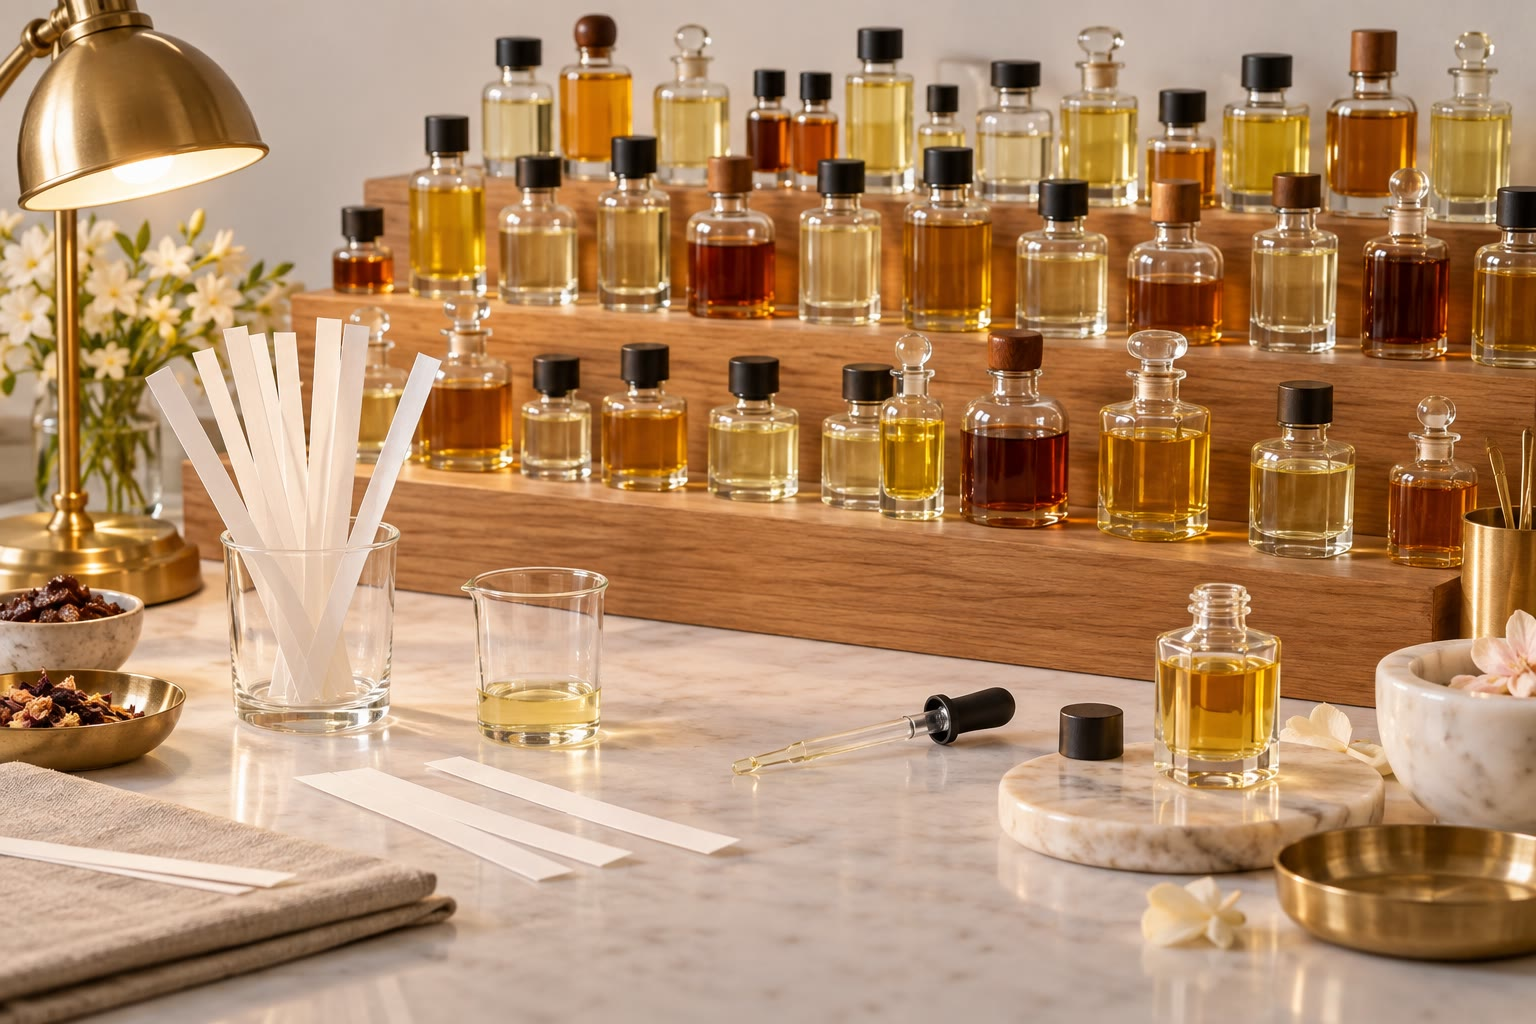
\includegraphics[width=0.48\linewidth]{images/book1/ai/g11-perfumer-lab.jpg}

{\small इत्र बनाने वाले की बेंच: बहुत-सी शीशियों में \omterm{def:g11:functional-groups:carboxylic-acid}{एस्टर}, \omterm{def:g11:functional-groups:alcohol}{ऐल्कोहॉल},
\omterm{def:g11:functional-groups:carbonyl}{ऐल्डिहाइड} और \omterm{def:g11:functional-groups:carbonyl}{कीटोन} हैं।}
\end{omfigure}

\begin{safety}{\ghs[0.82cm]{GHS02}\ghs[0.82cm]{GHS05}\ghs[0.82cm]{GHS07}}
% ledger: ghs:acetone, ghs:acetic-acid
प्रोपेनोन अत्यधिक ज्वलनशील है और आँखों में जलन करता है; इसकी वाष्प
उनींदापन लाती है। शुद्ध एथेनोइक अम्ल ज्वलनशील है और त्वचा और आँखों को गंभीर
रूप से जलाता है; सिरका उसका तनु विलयन है।
गंधें कभी फ़्लास्क को सूँघकर नहीं परखी जातीं: वाष्प को हाथ से धीरे-धीरे नाक
की ओर पंखे की तरह झला जाता है, और केवल तब जब शिक्षक
कहें।
\end{safety}

\section{अभ्यास}


\begin{exercise}[$\star$]\label{exo:g11:functional-groups:1}
हर यौगिक का \omterm{def:g11:functional-groups:functional-group}{क्रियात्मक समूह} और परिवार बताइए:
\ce{CH3-CH2-CH2-OH}; \ce{CH3-CO-CH2-CH3}; \ce{CH3-CH2-COOH};
\ce{CH3-COO-CH3}; \ce{CH3-CH2-NH2}।
\end{exercise}

\begin{exercise}[$\star$]\label{exo:g11:functional-groups:2}
नाम बताइए: \ce{CH3-OH}; \ce{CH3-CH2-CH2-OH}; \ce{HCOOH}; \ce{CH3-CH2-CHO};
\ce{CH3-CO-CH3}।
\end{exercise}

\begin{exercise}[$\star$]\label{exo:g11:functional-groups:3}
हर यौगिक किस परिवार का है: ब्यूटेन-2-ऑल, पेंटेनैल, मेथिल
प्रोपेनोएट, प्रोपेनेमाइड, 2-ब्रोमोप्रोपेन, ब्यूट-1-ईन?
\end{exercise}

\begin{exercise}[$\star$]\label{exo:g11:functional-groups:4}
प्रोपेनैल और प्रोपेनोन के \omterm{def:g11:organic-skeletons:formulas}{अर्ध-संरचना सूत्र} लिखिए। इनमें से कौन
\omterm{def:g11:functional-groups:carbonyl}{ऐल्डिहाइड} है? आप कैसे पहचानते हैं?
\end{exercise}

\begin{exercise}[$\star$]\label{exo:g11:functional-groups:5}
प्रोपेन-1-ऑल, प्रोपेन-2-ऑल और 2-मेथिलप्रोपेन-2-ऑल की श्रेणी बताइए।
\end{exercise}

\begin{exercise}[$\star\star$]\label{exo:g11:functional-groups:6}
पेंटेन-3-ऑल, 2-मेथिलब्यूटेनोइक अम्ल, हेक्सेन-2-ओन और प्रोपिल एथेनोएट के
\omterm{def:g11:organic-skeletons:formulas}{कंकाल सूत्र} बनाइए।
\end{exercise}

\begin{exercise}[$\star\star$]\label{exo:g11:functional-groups:7}
प्रोपेनैल और प्रोपेनोन का \omterm{def:g11:organic-skeletons:formulas}{आण्विक सूत्र} एक ही है। उसे बताइए। क्या
वे \omterm{def:g11:organic-skeletons:isomer}{समावयवी} हैं? क्या उनका \omterm{def:g11:functional-groups:functional-group}{क्रियात्मक समूह} एक ही है?
\end{exercise}

\begin{exercise}[$\star\star$]\label{exo:g11:functional-groups:8}
उस \omterm{def:g11:functional-groups:carboxylic-acid}{एस्टर} का \omterm{def:g11:organic-skeletons:formulas}{अर्ध-संरचना सूत्र} और नाम लिखिए जिसका अम्ल भाग
मेथेनोइक अम्ल \ce{HCOOH} से और \omterm{def:g11:functional-groups:alcohol}{ऐल्कोहॉल} भाग एथेनॉल से आता है; फिर
एथेनोइक अम्ल और प्रोपेन-1-ऑल से बने \omterm{def:g11:functional-groups:carboxylic-acid}{एस्टर} का।
\end{exercise}

\begin{exercise}[$\star\star$]\label{exo:g11:functional-groups:9}
\omterm{def:g11:functional-groups:carboxylic-acid}{एस्टरों} \ce{CH3-COO-CH3}, \ce{CH3-CH2-COO-CH2-CH3} और
\ce{HCOO-CH3} के नाम बताइए, और बताइए कि हर एक किस अम्ल और किस \omterm{def:g11:functional-groups:alcohol}{ऐल्कोहॉल} से संबंधित है।
\end{exercise}

\begin{exercise}[$\star\star$]\label{exo:g11:functional-groups:10}
सूत्र \ce{C4H10O} वाले चारों \omterm{def:g11:functional-groups:alcohol}{ऐल्कोहॉल} बनाइए और उनके नाम बताइए, और हर एक की
श्रेणी बताइए।
\end{exercise}

\begin{exercise}[$\star\star$]\label{exo:g11:functional-groups:11}
समूहों की सारणी की मदद से: \ce{CH3-CO-NH2} का परिवार क्या है? \omterm{def:g11:functional-groups:halogenoalkane}{ऐल्कीन} के
नाम का अंत क्या होता है? किन परिवारों में ऐसा कार्बोनिल समूह होता है जिसके उसी
कार्बन पर ऑक्सीजन या नाइट्रोजन \omterm{def:g7:atoms-and-molecules:atom}{परमाणु} हो?
\end{exercise}

\begin{exercise}[$\star\star\star$]\label{exo:g11:functional-groups:12}
ऐस्पिरिन और पैरासिटामॉल के \omterm{def:g11:functional-groups:functional-group}{क्रियात्मक समूहों} पर घेरा लगाइए और उनके नाम बताइए।
(पैरासिटामॉल के वलय जैसे किसी वलय से सीधे आबंधित \ce{-OH} को
फ़ीनॉल समूह कहते हैं; उसका व्यवहार \omterm{def:g11:functional-groups:alcohol}{ऐल्कोहॉल} से अलग होता है।)
\begin{center}
\setchemfig{atom sep=1.6em}
\chemfig{*6(-=-(-COOH)=(-O-[:150]C(=[:90]O)-[:210]H_3C)-=)}
\qquad
\chemfig{*6((-OH)=-=(-N(-[2]H)-[7]C(=[6]O)-[1]CH_3)-=-)}
\\[2pt] \small ऐस्पिरिन \hspace{4.2cm} पैरासिटामॉल
\end{center}
\end{exercise}

\begin{exercise}[$\star\star\star$]\label{exo:g11:functional-groups:13}
% ledger: bp:C2H5OH, bp:CH3OCH3
एथेनॉल \ce{CH3-CH2-OH} और मेथॉक्सीमेथेन \ce{CH3-O-CH3} का \omterm{def:g11:organic-skeletons:formulas}{आण्विक सूत्र}
एक ही है। उसे बताइए। मेथॉक्सीमेथेन ऐसे परिवार का है जो
सारणी में नहीं है: ईथर। दोनों में से कौन अपने ही \omterm{def:g7:atoms-and-molecules:molecule}{अणुओं} के बीच \omterm{def:g11:polarity-and-cohesion:hydrogen-bond}{हाइड्रोजन आबंध} बना
सकता है? कौन ऊँचे ताप पर उबलता है (एक \qty{78}{\celsius} पर उबलता है,
दूसरा \qty{-25}{\celsius} पर)?
\end{exercise}

\begin{exercise}[$\star\star\star$]\label{exo:g11:functional-groups:14}
थकी हुई मांसपेशियों द्वारा बनने वाला लैक्टिक अम्ल
\chemfig{CH_3-CH(-[2]OH)-COOH} है। उसके दोनों \omterm{def:g11:functional-groups:functional-group}{क्रियात्मक समूहों} के नाम बताइए। जब
किसी \omterm{def:g7:atoms-and-molecules:molecule}{अणु} में एक अम्ल समूह और एक दूसरा समूह हो, तो अम्ल अंत देता है
और दूसरा समूह उपसर्ग बन जाता है (\ce{-OH} के लिए \emph{हाइड्रॉक्सी-},
\ce{-NH2} के लिए \emph{ऐमीनो-})। लैक्टिक अम्ल का नाम बताइए, फिर ग्लाइसीन,
\ce{H2N-CH2-COOH}, का।
\end{exercise}

\begin{exercise}[$\star\star\star$]\label{exo:g11:functional-groups:15}
\omterm{def:g4:air-a-mixture-of-gases:air}{हवा} में खुली छोड़ी गई वाइन सिरका बन जाती है: एथेनॉल, एथेनैल से होकर, एथेनोइक
अम्ल बन जाता है। तीनों यौगिकों के अर्ध-संरचना और \omterm{def:g11:organic-skeletons:formulas}{आण्विक सूत्र}
और उनके परिवार लिखिए। हर चरण पर सूत्र में क्या बदलता है?
\end{exercise}

\section{समस्या: फलों की सुगंध}

\begin{problem}[{सप्ताहांत समस्या --- एक सुगंध-रसायनज्ञ केले की गंध बनाती है:
मुख्य अणु का मोलर द्रव्यमान क्या है?}]
\label{pb:g11:functional-groups:1}
% ledger: aw:C, aw:H, aw:O
एक सुगंध-रसायनज्ञ की बेंच पर पाँच यौगिक हैं:
\begin{center}
\begin{tabular}{ll}
A & \chemfig{CH_3-C(=[2]O)-O-CH_2-CH_2-CH(-[2]CH_3)-CH_3} \\[16pt]
B & \chemfig{HO-CH_2-CH_2-CH(-[2]CH_3)-CH_3} \\[10pt]
C & \ce{CH3-COOH} \\
D & \ce{CH3-CH2-CH2-CH2-CH2-CHO} \\
E & \ce{CH3-CH2-CH2-COO-CH2-CH3}
\end{tabular}
\end{center}
A की गंध केले और नाशपाती वाली टॉफ़ियों जैसी है, B की माल्ट जैसी, C की सिरके जैसी, D की कटी
घास जैसी, E की अनानास जैसी।

\medskip
\noindent\textbf{भाग I --- समूह और परिवार।}
\begin{enumerate}
  \item हर यौगिक के \omterm{def:g11:functional-groups:functional-group}{क्रियात्मक समूह} का नाम बताइए।
  \item हर एक का परिवार बताइए।
  \item कौन-से यौगिक \omterm{def:g11:functional-groups:carboxylic-acid}{एस्टर} हैं? उनकी गंधें कैसी हैं?
  \item \omterm{def:g11:functional-groups:alcohol}{ऐल्कोहॉल} B की श्रेणी क्या है?
  \item D का \omterm{def:g11:organic-skeletons:formulas}{आण्विक सूत्र} बताइए, और D का कोई ऐसा \omterm{def:g11:organic-skeletons:isomer}{समावयवी} बनाइए जो
        \omterm{def:g11:functional-groups:carbonyl}{कीटोन} हो।
\end{enumerate}

\medskip
\noindent\textbf{भाग II --- नाम।}
\begin{enumerate}[resume]
  \item B का नाम बताइए (वह सबसे लंबी श्रृंखला खोजिए जिसमें \ce{-OH} वाला
        कार्बन हो)।
  \item C और D के नाम बताइए।
  \item E का नाम बताइए, और बताइए कि वह किस अम्ल और किस \omterm{def:g11:functional-groups:alcohol}{ऐल्कोहॉल} से संबंधित है।
  \item A का नाम, 3-मेथिलब्यूटिल एथेनोएट, समझाइए: कौन-सा भाग
        अम्ल से आता है, कौन-सा \omterm{def:g11:functional-groups:alcohol}{ऐल्कोहॉल} से?
\end{enumerate}

\medskip
\noindent\textbf{भाग III --- अम्ल और \omterm{def:g11:functional-groups:alcohol}{ऐल्कोहॉल} से।}
\begin{enumerate}[resume]
  \item बेंच के किन दो यौगिकों से A संबंधित है?
  \item A, B और C के \omterm{def:g11:organic-skeletons:formulas}{आण्विक सूत्र} बताइए।
  \item \omterm{def:g11:functional-groups:carboxylic-acid}{एस्टर} अपने अम्ल और अपने \omterm{def:g11:functional-groups:alcohol}{ऐल्कोहॉल} से एक छोटा \omterm{def:g7:atoms-and-molecules:molecule}{अणु} खोकर बनता है।
        सूत्रों की मदद से पता कीजिए कि कौन-सा।
  \item A बनने का समीकरण \omterm{def:g11:organic-skeletons:formulas}{आण्विक सूत्रों} में लिखिए,
        और जाँचिए कि वह संतुलित है।
\end{enumerate}

\medskip
\noindent\textbf{भाग IV --- \omterm{def:g10:the-mole:molar-mass}{मोलर द्रव्यमान}।}
\begin{enumerate}[resume]
  \item B और C के \omterm{def:g10:the-mole:molar-mass}{मोलर द्रव्यमान} निकालिए।
  \item प्रश्न 13 के समीकरण से A का \omterm{def:g10:the-mole:molar-mass}{मोलर द्रव्यमान} निकालिए।
  \item A का \omterm{def:g10:the-mole:molar-mass}{मोलर द्रव्यमान} सीधे उसके सूत्र से निकालिए, और
        तुलना कीजिए।
  \item फलों जैसी गंध वाले एक अज्ञात नमूने का \omterm{def:g10:the-mole:molar-mass}{मोलर द्रव्यमान} लगभग
        \qty{116}{g/mol} पाया जाता है। क्या वह A है या E?
  \item हेप्टेनोइक अम्ल, \ce{CH3-(CH2)5-COOH}, की गंध बासी है। दिखाइए कि वह
        A का \omterm{def:g11:organic-skeletons:isomer}{समावयवी} है। क्या केवल \omterm{def:g10:the-mole:molar-mass}{मोलर द्रव्यमान} किसी यौगिक को पहचान सकता है?
  \item रसायनज्ञ क्यों कहते हैं कि गंध जितनी कंकाल की है, उतनी ही \omterm{def:g11:functional-groups:functional-group}{क्रियात्मक समूह}
        की भी? A और हेप्टेनोइक अम्ल का उपयोग कीजिए।
  \item अंतिम उत्तर बताइए: केले वाले \omterm{def:g11:functional-groups:carboxylic-acid}{एस्टर}, 3-मेथिलब्यूटिल एथेनोएट, का \omterm{def:g10:the-mole:molar-mass}{मोलर
        द्रव्यमान} क्या है?
\end{enumerate}
\end{problem}
